\begin{figure}[H]
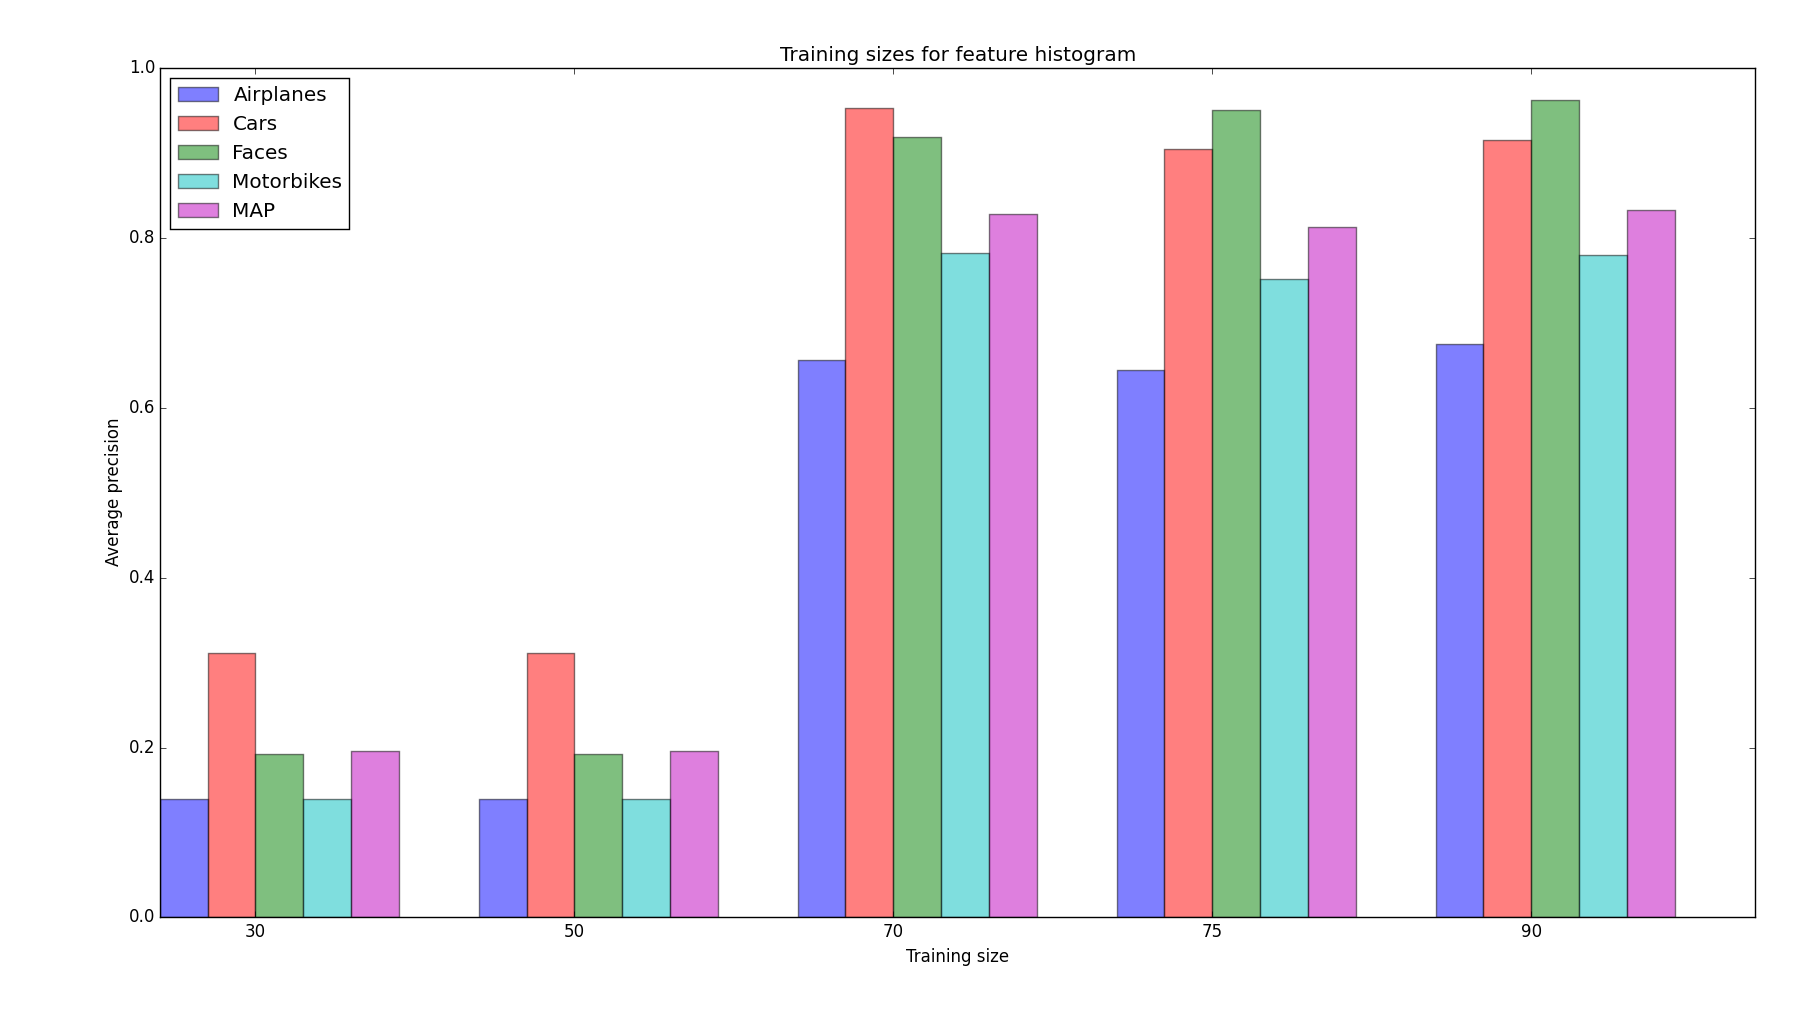
\includegraphics[width=\textwidth]{../plots/training_size_feature_histograms}
\caption{Effect of training size for histograms on AP}
\end{figure}
\begin{table}[H]
\begin{tabular}{|c|ccccc|}
\hline
\textbf{Training samples} & \textbf{AP Airplanes} & \textbf{AP Cars} & \textbf{AP Faces} & \textbf{AP Motorbikes} & \textbf{MAP}\\
\hline
30 & 0.1394 & 0.3118& 0.1924& 0.1394 & 0.1958\\
50 & 0.1394 & 0.3118& 0.1924& 0.1394 & 0.1958\\
70 & 0.6563 & 0.9534 & 0.9191 & 0.7830 & 0.8280\\
75 & 0.6447 & 0.9053 & 0.9510 & 0.7516 & 0.8132\\
90 & 0.6749 & 0.9157 & 0.9631 & 0.7798 & 0.8334\\
\hline
\end{tabular}
\caption{Effect number of training samples (per class) for feature histogram, Sift type: dense, Color space: opponent}
\end{table}
